\documentclass[11pt,a4paper]{article}

% Template note:
% This report uses a single-column course-paper layout adapted from common
% online paper templates. The figure-heavy structure is compiled with XeLaTeX
% and uses fixed float placement so diagrams remain near the text that explains
% them.

\usepackage{fontspec}
\usepackage{xeCJK}
\IfFontExistsTF{TeX Gyre Termes}{\setmainfont{TeX Gyre Termes}}{\setmainfont{Times New Roman}}
\IfFontExistsTF{Songti SC}{\setCJKmainfont{Songti SC}}{\setCJKmainfont{FandolSong-Regular}}
\IfFontExistsTF{Menlo}{\setmonofont{Menlo}}{\setmonofont{Latin Modern Mono}}
\IfFontExistsTF{Songti SC}{\setCJKmonofont{Songti SC}}{\setCJKmonofont{FandolSong-Regular}}
\usepackage[margin=24mm]{geometry}
\usepackage{amsmath,amssymb,mathtools}
\usepackage{booktabs}
\usepackage{array}
\usepackage{tabularx}
\usepackage{xcolor}
\usepackage{graphicx}
\usepackage{adjustbox}
\usepackage{tikz}
\usepackage{pgfplots}
\usepackage{algorithm}
\usepackage{algpseudocode}
\usepackage{listings}
\usepackage{enumitem}
\usepackage{float}
\usepackage{caption}
\usepackage{placeins}
\usepackage{url}
\usepackage[hidelinks]{hyperref}
\graphicspath{{figures/}}

\usetikzlibrary{arrows.meta,positioning,fit,calc,shapes.geometric,shapes.misc,shapes.symbols,backgrounds}
\pgfplotsset{compat=1.18}

\definecolor{scblue}{HTML}{1F6FEB}
\definecolor{scgreen}{HTML}{22A06B}
\definecolor{scorange}{HTML}{F59E0B}
\definecolor{scred}{HTML}{D1242F}
\definecolor{scgray}{HTML}{57606A}
\definecolor{sclight}{HTML}{F6F8FA}
\definecolor{scpurple}{HTML}{8250DF}

\setlength{\parskip}{0.35em}
\setlength{\parindent}{2em}
\captionsetup{font=small,labelfont=bf}
\captionsetup[table]{skip=5pt}
\newcommand{\reporttablesize}{\small}
\newcolumntype{Y}{>{\raggedright\arraybackslash}X}

\tikzset{
  box/.style={draw=scgray!45, rounded corners=2pt, fill=sclight, align=center, inner sep=5pt, font=\footnotesize},
  stage/.style={draw=scblue!70, fill=scblue!8, rounded corners=2pt, align=center, inner sep=5pt, font=\footnotesize\bfseries},
  data/.style={draw=scgreen!70, fill=scgreen!8, cylinder, shape border rotate=90, aspect=0.25, align=center, inner sep=5pt, font=\footnotesize},
  api/.style={draw=scorange!80, fill=scorange!12, rounded corners=2pt, align=center, inner sep=5pt, font=\footnotesize},
  model/.style={draw=scpurple!80, fill=scpurple!10, rounded corners=2pt, align=center, inner sep=5pt, font=\footnotesize},
  warn/.style={draw=scred!70, fill=scred!8, rounded corners=2pt, align=center, inner sep=5pt, font=\footnotesize},
  arrow/.style={-{Latex[length=2.0mm]}, thick, draw=scgray},
  dashedarrow/.style={-{Latex[length=2.0mm]}, thick, draw=scgray, dashed}
}

\lstset{
  basicstyle=\ttfamily\scriptsize,
  breaklines=true,
  frame=single,
  columns=fullflexible,
  backgroundcolor=\color{sclight},
  rulecolor=\color{scgray!35}
}

\title{SepsisCare：面向 ICU 脓毒症风险分层、动态表型学习与多端软件交付的课程项目报告}

\author{项目负责人：汪瑞可\\
Python 高级程序设计课程项目\\
本地演示系统版本 0.9.1，模型版本 S7-contrastive-20260516\\
\href{mailto:wangrk2023@shanghaitech.edu.cn}{wangrk2023@shanghaitech.edu.cn}}

\date{2026年6月3日（含 2026-05-30 至 2026-06-03 安全与部署增补）}

\begin{document}
\maketitle

\begin{abstract}
SepsisCare 是一个从 ICU 时间序列研究原型扩展到可安装软件系统的课程项目。项目目标不是替代临床诊断，而是在脱敏 ICU 数据与本地演示模型的基础上，展示脓毒症风险分层、动态表型轨迹、历史相似病例检索、家属沟通智能体与模型训练运维终端的端到端工程闭环。研究部分采用 PhysioNet 2012、PhysioNet 2019、MIMIC-IV 与 eICU 四类 ICU 数据源，形成从 S0 数据标准化到 S7 多源训练的迭代方法链。最终模型采用缺失感知 GRU 轨迹编码器、源均衡采样、GroupDRO 源目标、表型交叉熵与监督对比正则，最终在课程演示监控切分上达到宏平均 F1 0.956、编码器单独读出宏平均 F1 0.971、死亡 AUROC 0.848、下一时段机械通气 AUROC 0.968、剩余 ICU 住院时长 MAE 2.955 小时。工程部分交付 macOS、Windows、Android 安装包与独立云端模型部署包，后端通过标准 HTTP API 将本地/云端模型、DeepSeek 智能体、训练终端与多端客户端连接为一个可演示系统。2026 年 5 月 30 日之后，项目又补充了远端 Bearer token 鉴权、SSRF 防护、Web token 会话化、HTML 输出转义、运行时数据审计、敏感发布面审计、训练元数据完整性审计、artifact 清单校验和预发布安全门禁，使部署路径从“可运行演示”提升为“有安全边界、有污染检查、有复现证据的交付流程”。
\end{abstract}

\noindent\textbf{关键词：}
脓毒症，ICU 时间序列，动态表型，缺失感知 GRU，GroupDRO，监督对比学习，Electron，SwiftUI，Android WebView，DeepSeek，软件工程交付

\section{背景与问题定义}
\subsection{临床与课程项目背景}
脓毒症是 ICU 常见高风险综合征之一，其状态变化快、器官系统参与复杂，单一时刻的静态风险评分难以完整表达患者在 48 小时内的轨迹演化。课程项目需要同时体现算法研究、软件工程与可交付安装包三类能力，因此 SepsisCare 将问题拆成两个层面：
\begin{enumerate}[leftmargin=*,itemsep=1pt]
  \item \textbf{研究层面：}从 ICU 时间序列中学习稳定、可解释、可迁移的动态表型与风险表示。
  \item \textbf{工程层面：}把研究原型封装成医生端、研究端、家属端、管理员端、训练终端可共同访问的软件系统。
\end{enumerate}

系统最终不声称达到临床投产验证标准。所有演示输出均标注为课程演示、脱敏数据和辅助沟通用途；正式生产需要外部伦理审批、真实医院部署、独立外部验证、模型监管和安全审计。

\subsection{任务定义}
给定 ICU 患者在前 48 小时内的多变量时间序列：
\begin{equation}
  X_i=\{x_{i,t}\in\mathbb{R}^{F}\}_{t=1}^{48},\quad
  M_i=\{m_{i,t}\in\{0,1\}^{F}\}_{t=1}^{48},
\end{equation}
其中 $M_i$ 为观测掩码，目标是学习患者级表示 $z_i$ 与窗口级表示 $z_{i,w}$，支持以下输出：
\begin{align}
  \hat{y}^{mort}_i &= f_{mort}(z_i),\\
  \hat{c}_{i,w} &= f_{phenotype}(z_{i,w}),\\
  \hat{y}^{mv}_{i,w+1} &= f_{mv}(z_{i,w}),\\
  \widehat{\log(1+\mathrm{LOS})}_{i,w} &= f_{los}(z_{i,w}).
\end{align}
其中 $\hat{c}_{i,w}$ 是 24 小时滚动窗口的表型标签，用于解释疾病状态轨迹。

\begin{figure}[H]
\centering
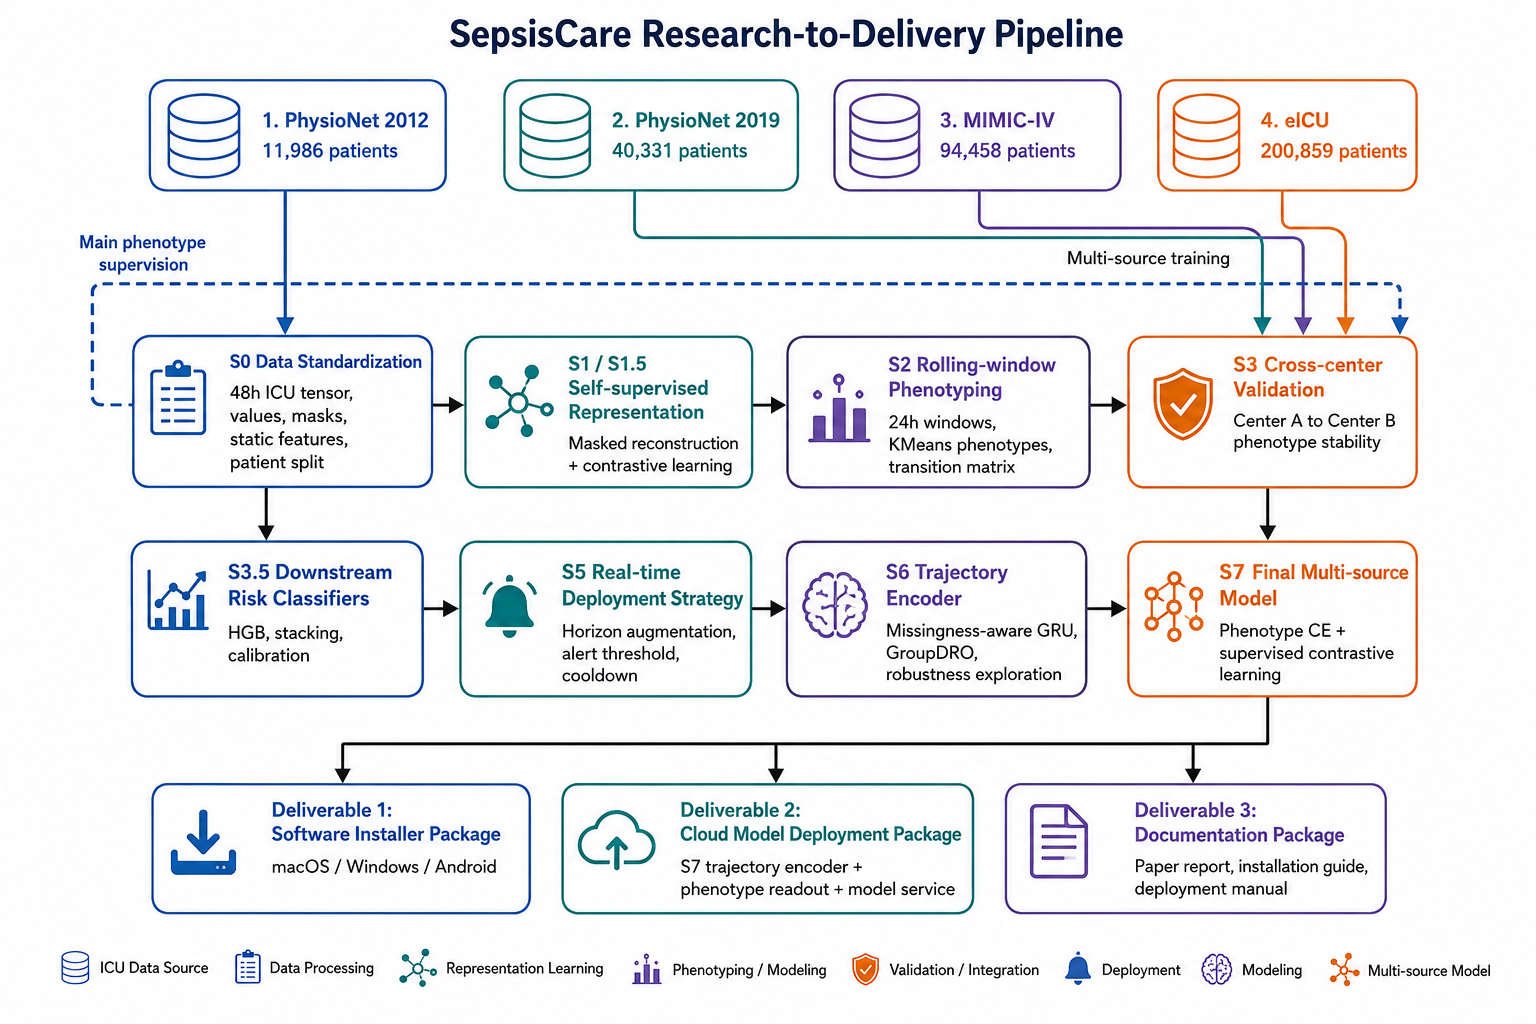
\includegraphics[width=\textwidth]{fig1_pipeline.png}
\caption{\textbf{SepsisCare 从研究流水线到最终交付物的总体图。} 图中上方四个数据库表示本项目使用的 ICU 数据来源：PhysioNet 2012 作为主表型监督来源，PhysioNet 2019、MIMIC-IV 与 eICU 作为跨源训练和鲁棒性验证来源。中间的 S0--S7 表示完整方法迭代链：先将原始 ICU 记录标准化为 48 小时张量，再通过自监督表示学习、滚动窗口表型、跨中心验证、实时部署校准、缺失感知 GRU 和多源表型监督训练逐步形成最终模型。底部三类交付物对应课程项目最终输出：软件安装包、云端模型部署包和完整说明文档。}
\label{fig:global-pipeline}
\end{figure}

\section{数据集选择}
\subsection{选择原则}
数据集选择遵循四个原则：第一，必须具备 ICU 时间序列；第二，应覆盖不同医院或数据库来源；第三，需要能映射到 48 小时窗口；第四，课程交付包只包含脱敏演示数据和模型报告，不包含受限原始数据库。

\begin{table}[H]
\centering
\caption{主要数据源及其在项目中的角色}
\label{tab:datasets}
\reporttablesize
\setlength{\tabcolsep}{5pt}
\renewcommand{\arraystretch}{1.12}
\begin{tabularx}{\textwidth}{@{}l r l Y@{}}
\toprule
数据源 & 样本量 & 项目角色 & 关键用途\\
\midrule
PhysioNet 2012 & 11,986 & 主源 & S0--S3 表型、S6/S7 主表型监督\\
PhysioNet 2019 & 40,331 & 辅助源 & sepsis 标签、跨源辅助任务\\
MIMIC-IV & 94,458 & 外部源 & 多源训练、MIMIC 迁移验证\\
eICU & 200,859 & 外部源 & 多中心大样本辅助任务、鲁棒性压力测试\\
\midrule
合计 & 347,634 & S7 训练监控 & 全源训练与交付模型报告\\
\bottomrule
\end{tabularx}
\end{table}

\subsection{S0 统一表示}
所有来源被尽量映射到统一的 48 小时 ICU 张量接口：
\begin{equation}
  \mathcal{D}^{(s)}=\{X^{(s)},M^{(s)},P^{(s)},A^{(s)},Y^{(s)}\},
\end{equation}
其中 $P$ 表示代理/干预特征，$A$ 表示静态特征，$Y$ 表示可用结局。S7 训练中主源和外部源的可用标签不完全一致，因此损失函数采用掩码形式：
\begin{equation}
  \mathcal{L}_{task}
  =
  \sum_{k\in\mathcal{K}}
  \lambda_k
  \frac{\sum_i r_{ik}\ell_k(\hat{y}_{ik},y_{ik})}{\sum_i r_{ik}+\epsilon},
\end{equation}
其中 $r_{ik}=1$ 表示样本 $i$ 具有任务 $k$ 的标签。

\section{S0 到 S7 的方法选择}
\subsection{S0：数据清洗、标准化与切分}
S0 将小时级 ICU 数据变换为张量。连续特征使用训练集统计量标准化：
\begin{equation}
  \tilde{x}_{i,t,f}=\frac{x_{i,t,f}-\mu_f^{train}}{\sigma_f^{train}+\epsilon}.
\end{equation}
缺失值通过掩码保留，必要时使用训练集均值或前向填充形成模型输入。患者级切分避免同一患者跨训练和测试泄漏。

\begin{algorithm}[H]
\caption{S0 统一 ICU 张量构建}
\label{alg:s0}
\begin{algorithmic}[1]
\Require 原始 ICU 表格、变量映射表、48h 窗口定义
\Ensure $X,M,A,Y$ 与 patient-level splits
\For{每个患者 $i$}
  \State 对齐入 ICU 后 $1,\ldots,48$ 小时
  \State 将生命体征、实验室指标、治疗事件映射到统一字段
  \State 生成观测掩码 $M_i$ 与连续矩阵 $X_i$
\EndFor
\State 仅在训练患者上估计 $\mu_f,\sigma_f$
\State 标准化 $X$，保存 preprocessing statistics
\State 输出 train/val/test 患者级切分
\end{algorithmic}
\end{algorithm}

\subsection{S1：Masked Reconstruction 表示学习}
S1 使用 Transformer 编码器学习静态 48 小时序列表示。随机掩盖观测位置集合 $\Omega$，优化重构损失：
\begin{equation}
  \mathcal{L}_{rec}
  =
  \frac{1}{|\Omega|}
  \sum_{(i,t,f)\in\Omega}
  \left(\hat{x}_{i,t,f}-\tilde{x}_{i,t,f}\right)^2.
\end{equation}
该阶段的意义是利用无监督结构学习 ICU 轨迹，但早期结果显示 PCA 在死亡率分离上仍有竞争力，因此进入 S1.5。

\subsection{S1.5：对比增强的自监督学习}
S1.5 在 masked reconstruction 外加入同一患者随机窗口增强的 NT-Xent 损失。对同一患者两种增强视图 $a,b$：
\begin{equation}
  \ell_{i}^{con}
  =
  -\log
  \frac{\exp(\mathrm{sim}(z_i^a,z_i^b)/\tau)}
  {\sum_{j}\mathbf{1}_{j\neq i}\exp(\mathrm{sim}(z_i^a,z_j)/\tau)}.
\end{equation}
总损失为：
\begin{equation}
  \mathcal{L}_{S1.5}=\mathcal{L}_{rec}+\lambda(t)\mathcal{L}_{con},
  \quad \lambda(t):0\rightarrow 0.5.
\end{equation}
S1.5 在 K=4 表型中兼顾几何聚类与死亡率分离，被用于后续滚动窗口表型。

\subsection{S2：滚动窗口表型与转移矩阵}
S2 将每个患者分解为 5 个滚动窗口：
\begin{equation}
  W=\{[0,24),[6,30),[12,36),[18,42),[24,48)\}.
\end{equation}
对每个窗口编码 $z_{i,w}=g_\theta(X_{i,w},M_{i,w})$ 后，在训练窗口上拟合 KMeans：
\begin{equation}
  \min_{\{\mu_k\}}\sum_{i,w}\min_{k\in\{1,\ldots,K\}}\|z_{i,w}-\mu_k\|_2^2.
\end{equation}
经验转移矩阵采用 Laplace 平滑：
\begin{equation}
  T_{ab}=
  \frac{N(c_w=a,c_{w+1}=b)+\alpha}
  {\sum_{b'}N(c_w=a,c_{w+1}=b')+K\alpha}.
\end{equation}
该阶段发现 P2 是最高风险稳定表型，Center A 到 Center B 的 6 项跨中心标准全部通过。

\subsection{S3：跨中心验证}
S3 将 Center A 上训练得到的编码器与 KMeans 表型直接应用于 Center B，比较稳定比例、非自转移比例、死亡率排序、最高风险表型、死亡率范围和 prevalence L1。验证通过意味着表型结构不是单一中心噪声。

\begin{figure}[H]
\centering
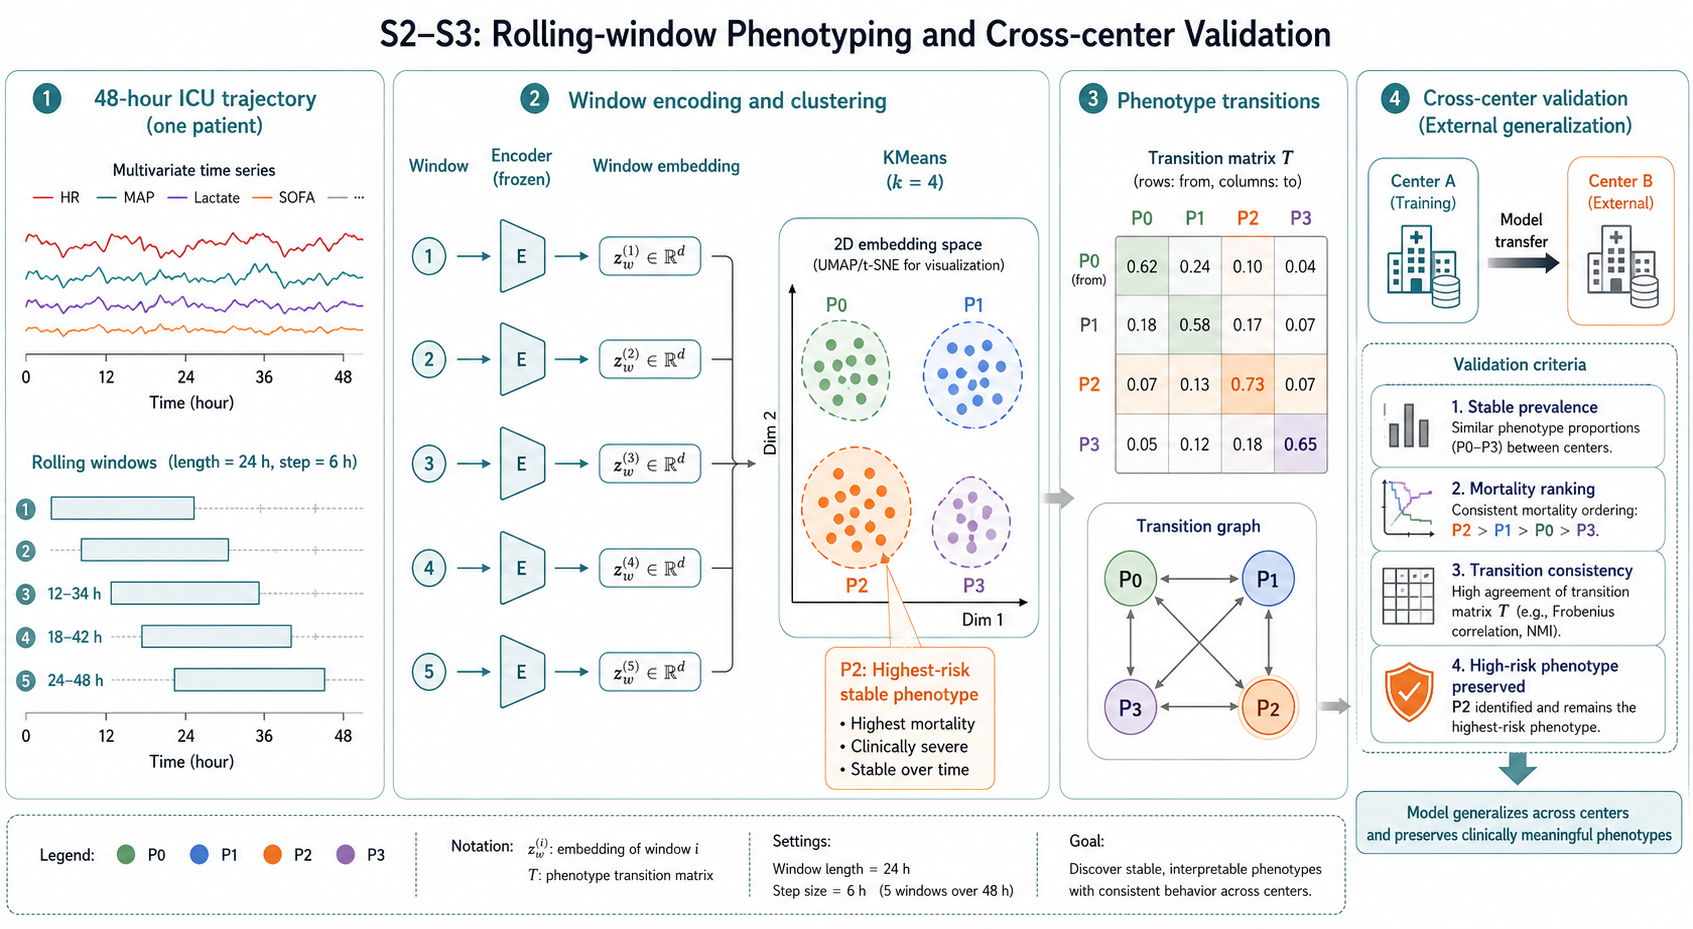
\includegraphics[width=\textwidth]{fig2_s2_s3.png}
\caption{\textbf{S2--S3 滚动窗口表型发现与跨中心验证流程。} 左侧展示单个 ICU 患者 48 小时多变量轨迹被切分为 5 个长度为 24 小时、步长为 6 小时的滚动窗口；每个窗口经冻结编码器映射为窗口嵌入 $z_w$，随后通过 KMeans 聚为 P0--P3 四类动态表型。中间部分展示表型间的经验转移矩阵 $T$ 和状态转移图，其中 P2 被标记为最高风险且相对稳定的表型。右侧展示 Center A 到 Center B 的外部迁移验证逻辑，通过 prevalence 稳定性、死亡率排序、转移一致性和最高风险表型保留来判断表型是否具有跨中心泛化意义。}
\label{fig:s2-s3-phenotyping}
\end{figure}

\subsection{S3.5：下游死亡风险分类与校准}
S3.5 将 S1.5 表示与统计特征组合，比较 Logistic Regression、HistGradientBoosting、OOF stacking 与校准方法。二分类交叉熵为：
\begin{equation}
  \mathcal{L}_{BCE}=-y\log p-(1-y)\log(1-p).
\end{equation}
温度校准形式为：
\begin{equation}
  p_T=\sigma\left(\frac{\mathrm{logit}(p)}{T}\right).
\end{equation}
该阶段最佳 calibrated stacking 的 AUROC 约 0.873，验证了表征可支持风险排序。

\subsection{S5：实时部署策略与 Horizon Augmentation}
部署场景中，模型在第 $h$ 小时只能看到 $h$ 小时真实数据。S5 引入 horizon augmentation，在训练时随机截断：
\begin{equation}
  h\sim \mathrm{Uniform}\{h_{min},\ldots,48\},\quad
  X_{t>h}=0,\ M_{t>h}=0.
\end{equation}
策略层使用阈值、最小历史长度、连续触发、冷却时间等规则控制报警：
\begin{equation}
  a_{i,h}=\mathbf{1}\{p_{i,h}\geq \theta_{enter},\ h\geq h_{min},\ c_{i,h}\geq c_{min}\}.
\end{equation}
该阶段将 MIMIC 早期负例过报警问题从不可用策略修复为可演示策略。

\subsection{S6：轨迹编码器、缺失感知和跨源鲁棒性探索}
S6 从表型一致性角度训练 GRU 轨迹编码器。输入包含连续值、掩码、代理特征和缺失时间差：
\begin{equation}
  \delta_{t,f}=\min(\delta_{t-1,f}+1,48)\cdot(1-m_{t,f}),
  \quad u_t=[\tilde{x}_t,m_t,p_t,\delta_t].
\end{equation}
GRU 更新：
\begin{align}
  r_t&=\sigma(W_r u_t+U_r h_{t-1}),\\
  q_t&=\sigma(W_q u_t+U_q h_{t-1}),\\
  \tilde{h}_t&=\tanh(W_h u_t+U_h(r_t\odot h_{t-1})),\\
  h_t&=(1-q_t)\odot h_{t-1}+q_t\odot\tilde{h}_t.
\end{align}
辅助任务包括死亡、sepsis、LOS、下一时段机械通气和 RRT。候选方案包括 S19 辅助预训练、DANN/CORAL、GroupDRO、GRU-D、温度集成。最终证据显示缺失感知 GroupDRO 对 MIMIC 有帮助，但 eICU 仍是更难的域。

\subsection{S7：最终多源表型监督模型}
S7 将所有可配置来源纳入训练，采用源均衡采样、GroupDRO 和主源表型监督。每个 step 从来源集合 $\mathcal{S}$ 中均衡采样 batch，计算每源损失 $L_s$。GroupDRO 权重更新为：
\begin{equation}
  q_s \leftarrow \frac{q_s\exp(\eta L_s)}{\sum_{s'}q_{s'}\exp(\eta L_{s'})},
  \quad
  \mathcal{L}_{GDRO}=\sum_s q_sL_s.
\end{equation}
主源表型交叉熵：
\begin{equation}
  \mathcal{L}_{phenCE}
  =
  -\frac{1}{N}\sum_i\sum_{k=1}^{K} \mathbf{1}(c_i=k)\log p_{ik}.
\end{equation}
监督对比损失为：
\begin{equation}
  \mathcal{L}_{SupCon}
  =
  \sum_i
  \frac{-1}{|P(i)|}
  \sum_{p\in P(i)}
  \log
  \frac{\exp(z_i^\top z_p/\tau)}
  {\sum_{a\neq i}\exp(z_i^\top z_a/\tau)}.
\end{equation}
最终目标：
\begin{equation}
\begin{split}
  \mathcal{L}_{S7}=&\mathcal{L}_{GDRO}
  +\lambda_{phen}\mathcal{L}_{phenCE}
  +\lambda_{sup}\mathcal{L}_{SupCon}\\
  &+\lambda_{los}\mathcal{L}_{LOS}
  +\lambda_{mv}\mathcal{L}_{MV}
  +\lambda_{rrt}\mathcal{L}_{RRT}.
\end{split}
\end{equation}

\begin{figure}[H]
\centering
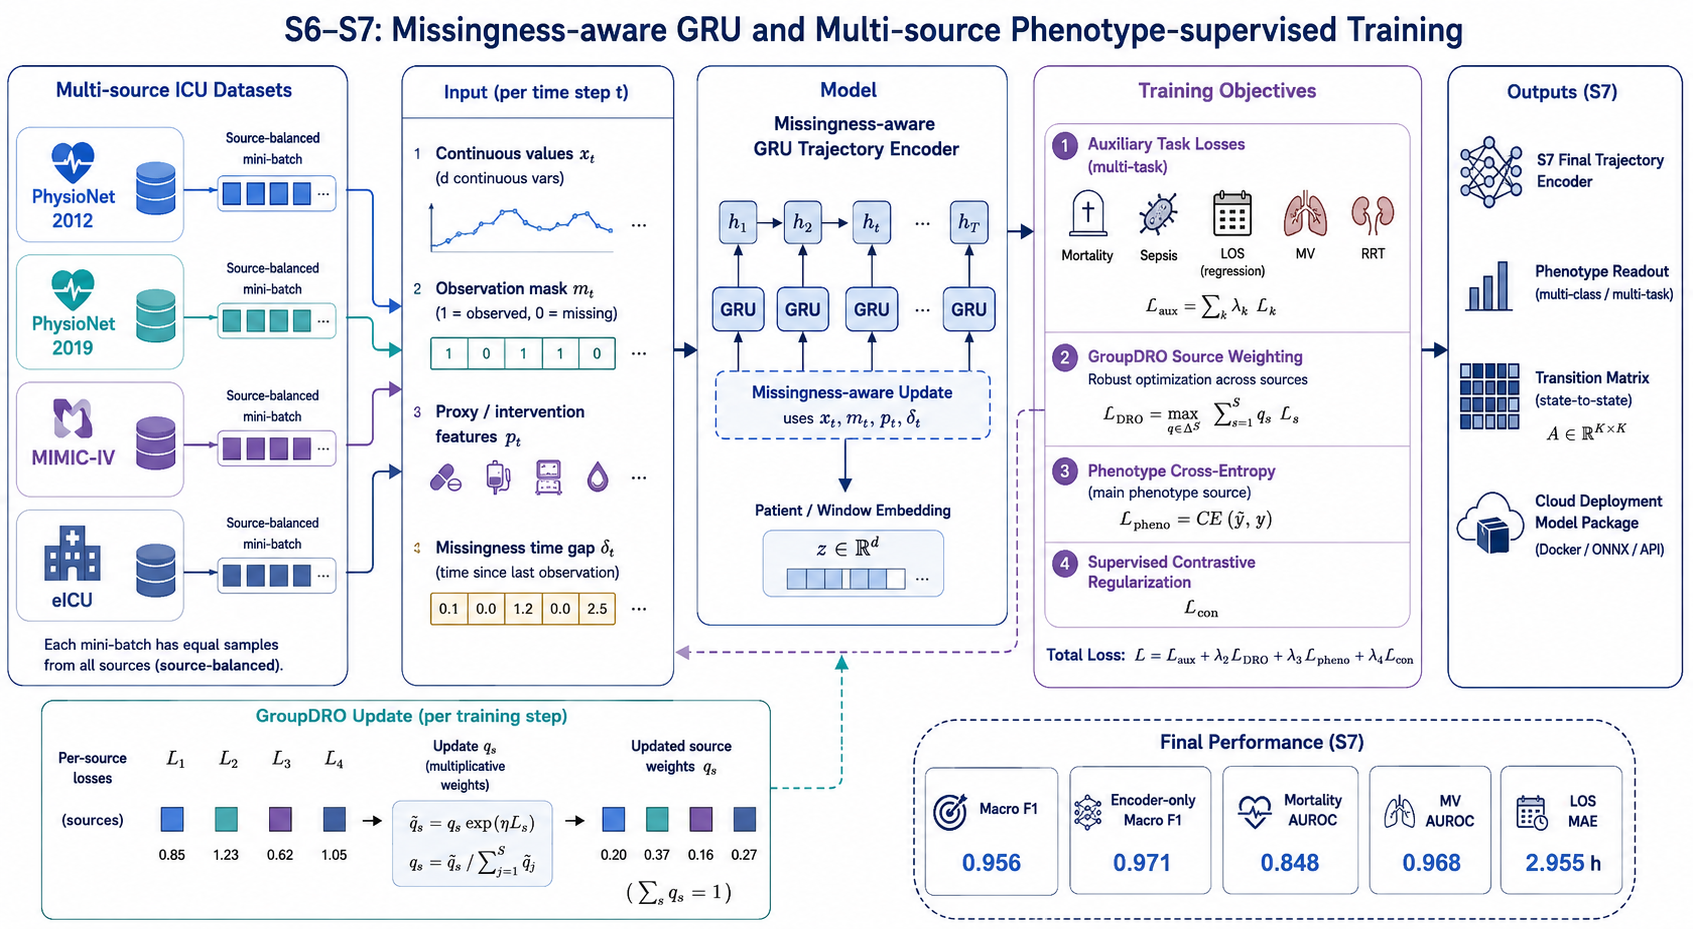
\includegraphics[width=\textwidth]{fig3_s6_s7.png}
\caption{\textbf{S6--S7 缺失感知 GRU 与多源表型监督训练框架。} 左侧四个来源通过 source-balanced mini-batch 进入统一训练过程，避免某一数据库因样本量或采样频率差异主导梯度。输入层同时包含连续变量 $x_t$、观测掩码 $m_t$、代理/干预特征 $p_t$ 与距离上次观测的缺失时间差 $\delta_t$，使轨迹编码器能够显式建模 ICU 数据的缺失机制。中间的 missingness-aware GRU 输出患者或窗口级嵌入 $z$；训练目标由辅助任务损失、GroupDRO 来源权重、主源表型交叉熵和监督对比正则共同组成。右侧对应最终 S7 输出，包括轨迹编码器、表型读出器、状态转移矩阵和可部署模型包；底部列出课程演示监控切分上的关键指标，用于说明最终模型在表型一致性、死亡风险、机械通气预测和 LOS 估计上的综合能力。}
\label{fig:s6-s7-training}
\end{figure}

\begin{algorithm}[H]
\caption{S7 源均衡 GroupDRO + 表型监督训练}
\label{alg:s7}
\begin{algorithmic}[1]
\Require 来源集合 $\mathcal{S}$，主源表型标签，辅助任务标签
\Ensure 轨迹编码器 $g_\theta$、表型读出器 $r_\phi$、转移矩阵 $T$
\State 初始化 GroupDRO 权重 $q_s=1/|\mathcal{S}|$
\For{epoch $=1,\ldots,E$}
  \For{step $=1,\ldots,B$}
    \For{每个来源 $s\in\mathcal{S}$}
      \State 采样 batch $B_s$，计算辅助任务损失 $L_s$
    \EndFor
    \State 更新 $q_s\propto q_s\exp(\eta L_s)$
    \State 在主源 batch 上计算 $\mathcal{L}_{phenCE}$ 与 $\mathcal{L}_{SupCon}$
    \State 反向传播 $\mathcal{L}_{S7}$
  \EndFor
\EndFor
\State 用主源 train 表型标签拟合读出器 $r_\phi$
\State 用主源 train 轨迹拟合 $T$
\end{algorithmic}
\end{algorithm}

\section{结果}
\subsection{主要实验结果}
\begin{table}[H]
\centering
\caption{最终 S7 模型主要监控结果}
\label{tab:s7-results}
\reporttablesize
\setlength{\tabcolsep}{8pt}
\renewcommand{\arraystretch}{1.12}
\begin{tabular}{@{}lr@{}}
\toprule
指标 & 数值\\
\midrule
训练来源总患者数 & 347,634\\
模型参数量 & 31,319\\
使用 GPU 数 & 7\\
Encoder-only window match & 0.972\\
Encoder-only Macro F1 & 0.971\\
Encoder + transition window match & 0.958\\
Encoder + transition Macro F1 & 0.956\\
Full-patient match rate & 0.832\\
Mortality AUROC & 0.848\\
Next mechanical ventilation AUROC & 0.968\\
Remaining LOS MAE & 2.955 h\\
\bottomrule
\end{tabular}
\end{table}

结果表明，最终 S7 模型在课程演示监控切分中能很好地复现 S2 表型轨迹，同时保留死亡、机械通气和 LOS 等辅助任务能力。需要强调的是，S7 监控切分故意与训练患者重叠，用于课程交付、模型比较和部署 smoke，不可写成独立 held-out 外部验证性能。

\subsection{关键消融结论}
\begin{enumerate}[leftmargin=*,itemsep=1pt]
  \item S1.5 对比学习提升了表示空间稳定性，但单独并不能解决所有外部域差异。
  \item S2 滚动窗口可发现有意义的动态表型，且在 PhysioNet 2012 Center A/B 上具备跨中心一致性。
  \item S6 的源均衡 DANN/CORAL 没有稳定改善 eICU，说明简单域不变约束会破坏部分表型信息。
  \item 缺失感知特征对 MIMIC 迁移有明显帮助，提示 ICU 数据源差异部分来自采样频率和缺失机制。
  \item S7 加入表型 CE 与 SupCon 后，课程演示表型一致性大幅提升，适合作为最终交付模型。
\end{enumerate}

\begin{figure}[H]
\centering
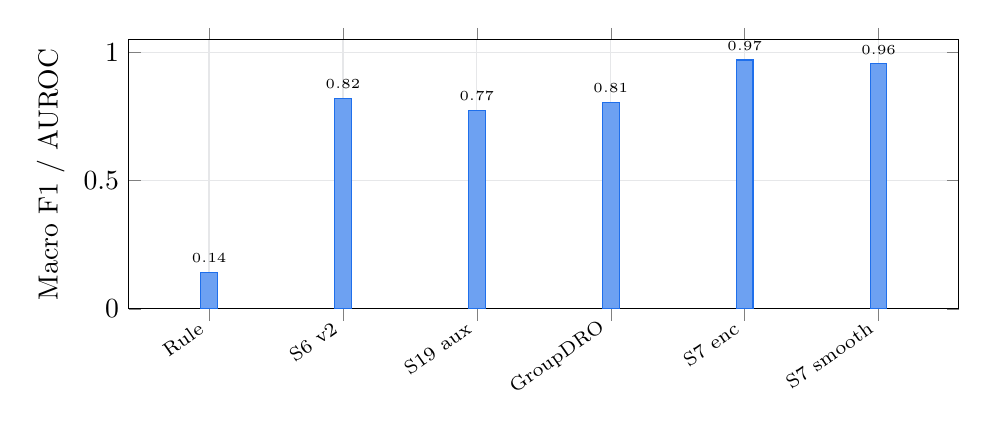
\begin{tikzpicture}
\begin{axis}[
  width=\columnwidth,
  height=50mm,
  ybar,
  ymin=0,
  ymax=1.05,
  ylabel={Macro F1 / AUROC},
  symbolic x coords={Rule,S6 v2,S19 aux,GroupDRO,S7 enc,S7 smooth},
  xtick=data,
  x tick label style={rotate=35,anchor=east,font=\scriptsize},
  nodes near coords,
  nodes near coords style={font=\tiny},
  bar width=6pt,
  enlarge x limits=0.12,
  grid=major,
  grid style={draw=scgray!15}
]
\addplot[fill=scblue!65,draw=scblue] coordinates {
  (Rule,0.142)
  (S6 v2,0.821)
  (S19 aux,0.773)
  (GroupDRO,0.806)
  (S7 enc,0.971)
  (S7 smooth,0.956)
};
\end{axis}
\end{tikzpicture}
\caption{表型一致性方法链的代表性指标。S7 enc/smooth 为最终模型在演示监控切分上的结果。}
\label{fig:metric-bars}
\end{figure}

\FloatBarrier
\section{软件工程系统结构}
\subsection{软件整体介绍}
SepsisCare 是一个面向课程演示与软件工程验收的 ICU 脓毒症辅助分析系统。客户端首屏以风险看板为核心，展示当前患者、48 小时实时趋势、风险解释和模型状态；研究端提供历史 ICU 病例库、相似病例检索、数据集摘要和模型实验记录；家属端接入 DeepSeek 智能体，用自然语言解释非诊断性病情信息；训练终端提供本地演示模式与云端生产模式切换，用于下发继续训练、暂停训练、下载权重、查看日志和同步配置等运维命令。

\begin{figure}[H]
\centering
\begin{minipage}{0.485\textwidth}
  \centering
  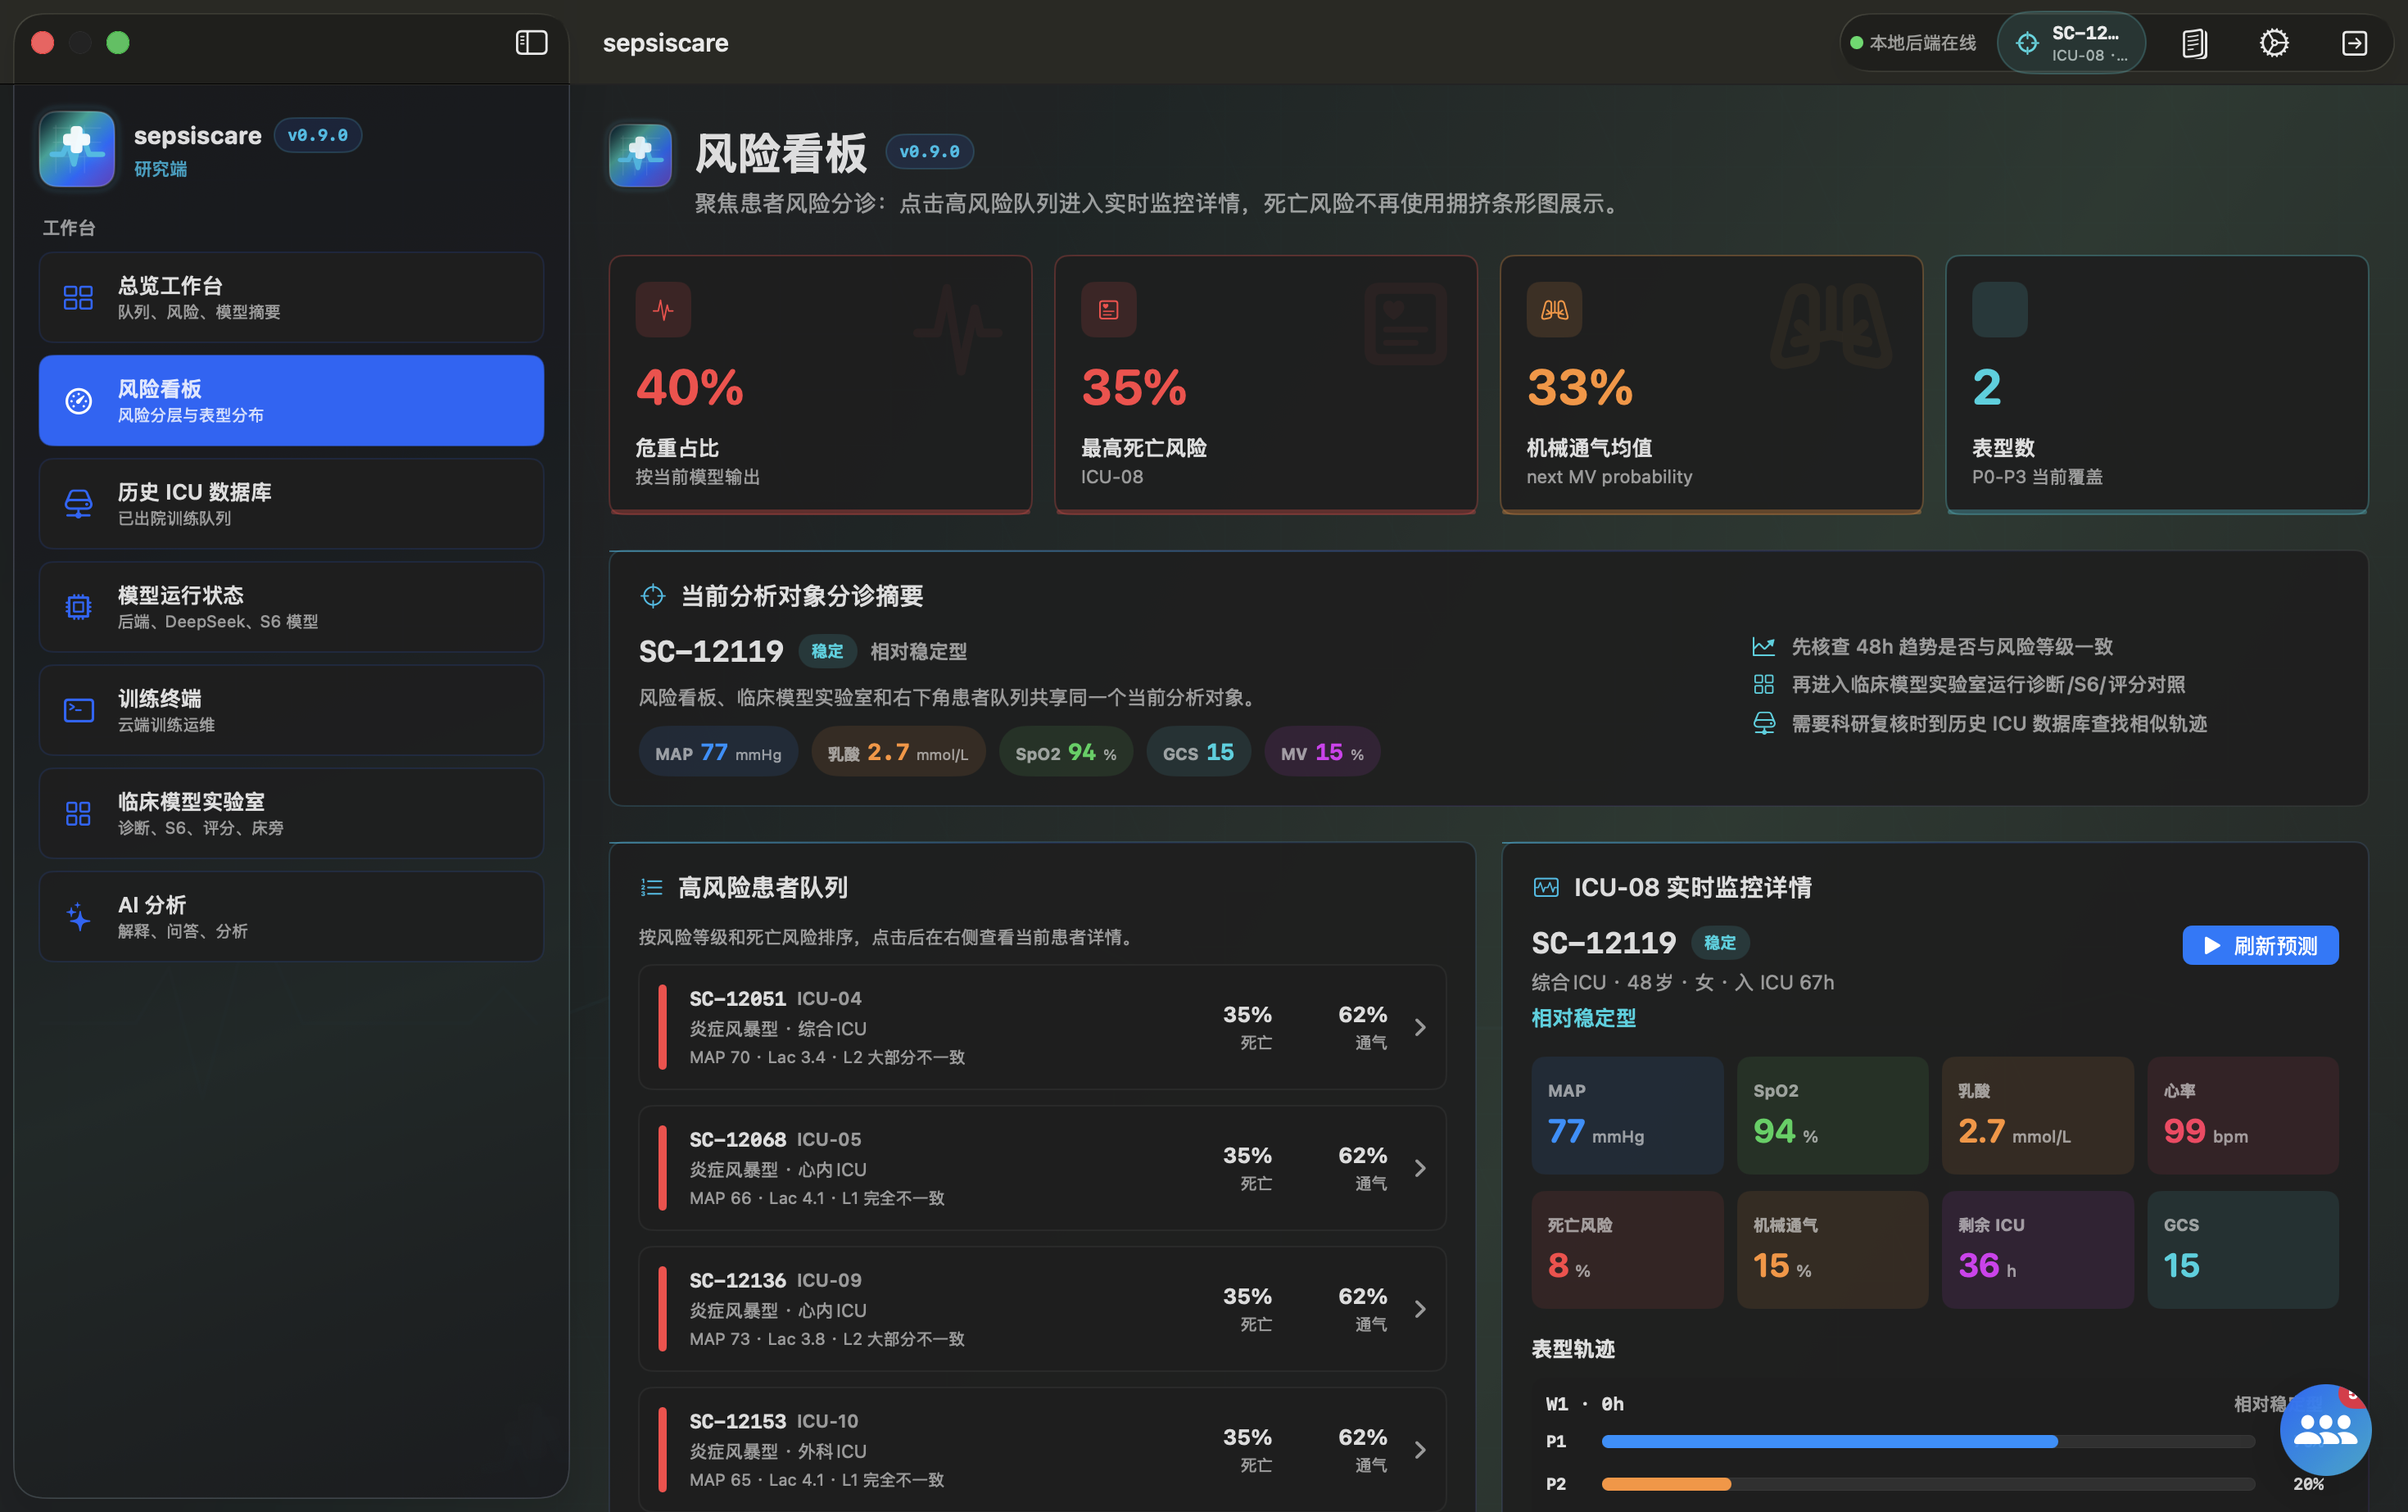
\includegraphics[width=\linewidth]{sepsiscareUI1.png}
\end{minipage}
\hfill
\begin{minipage}{0.485\textwidth}
  \centering
  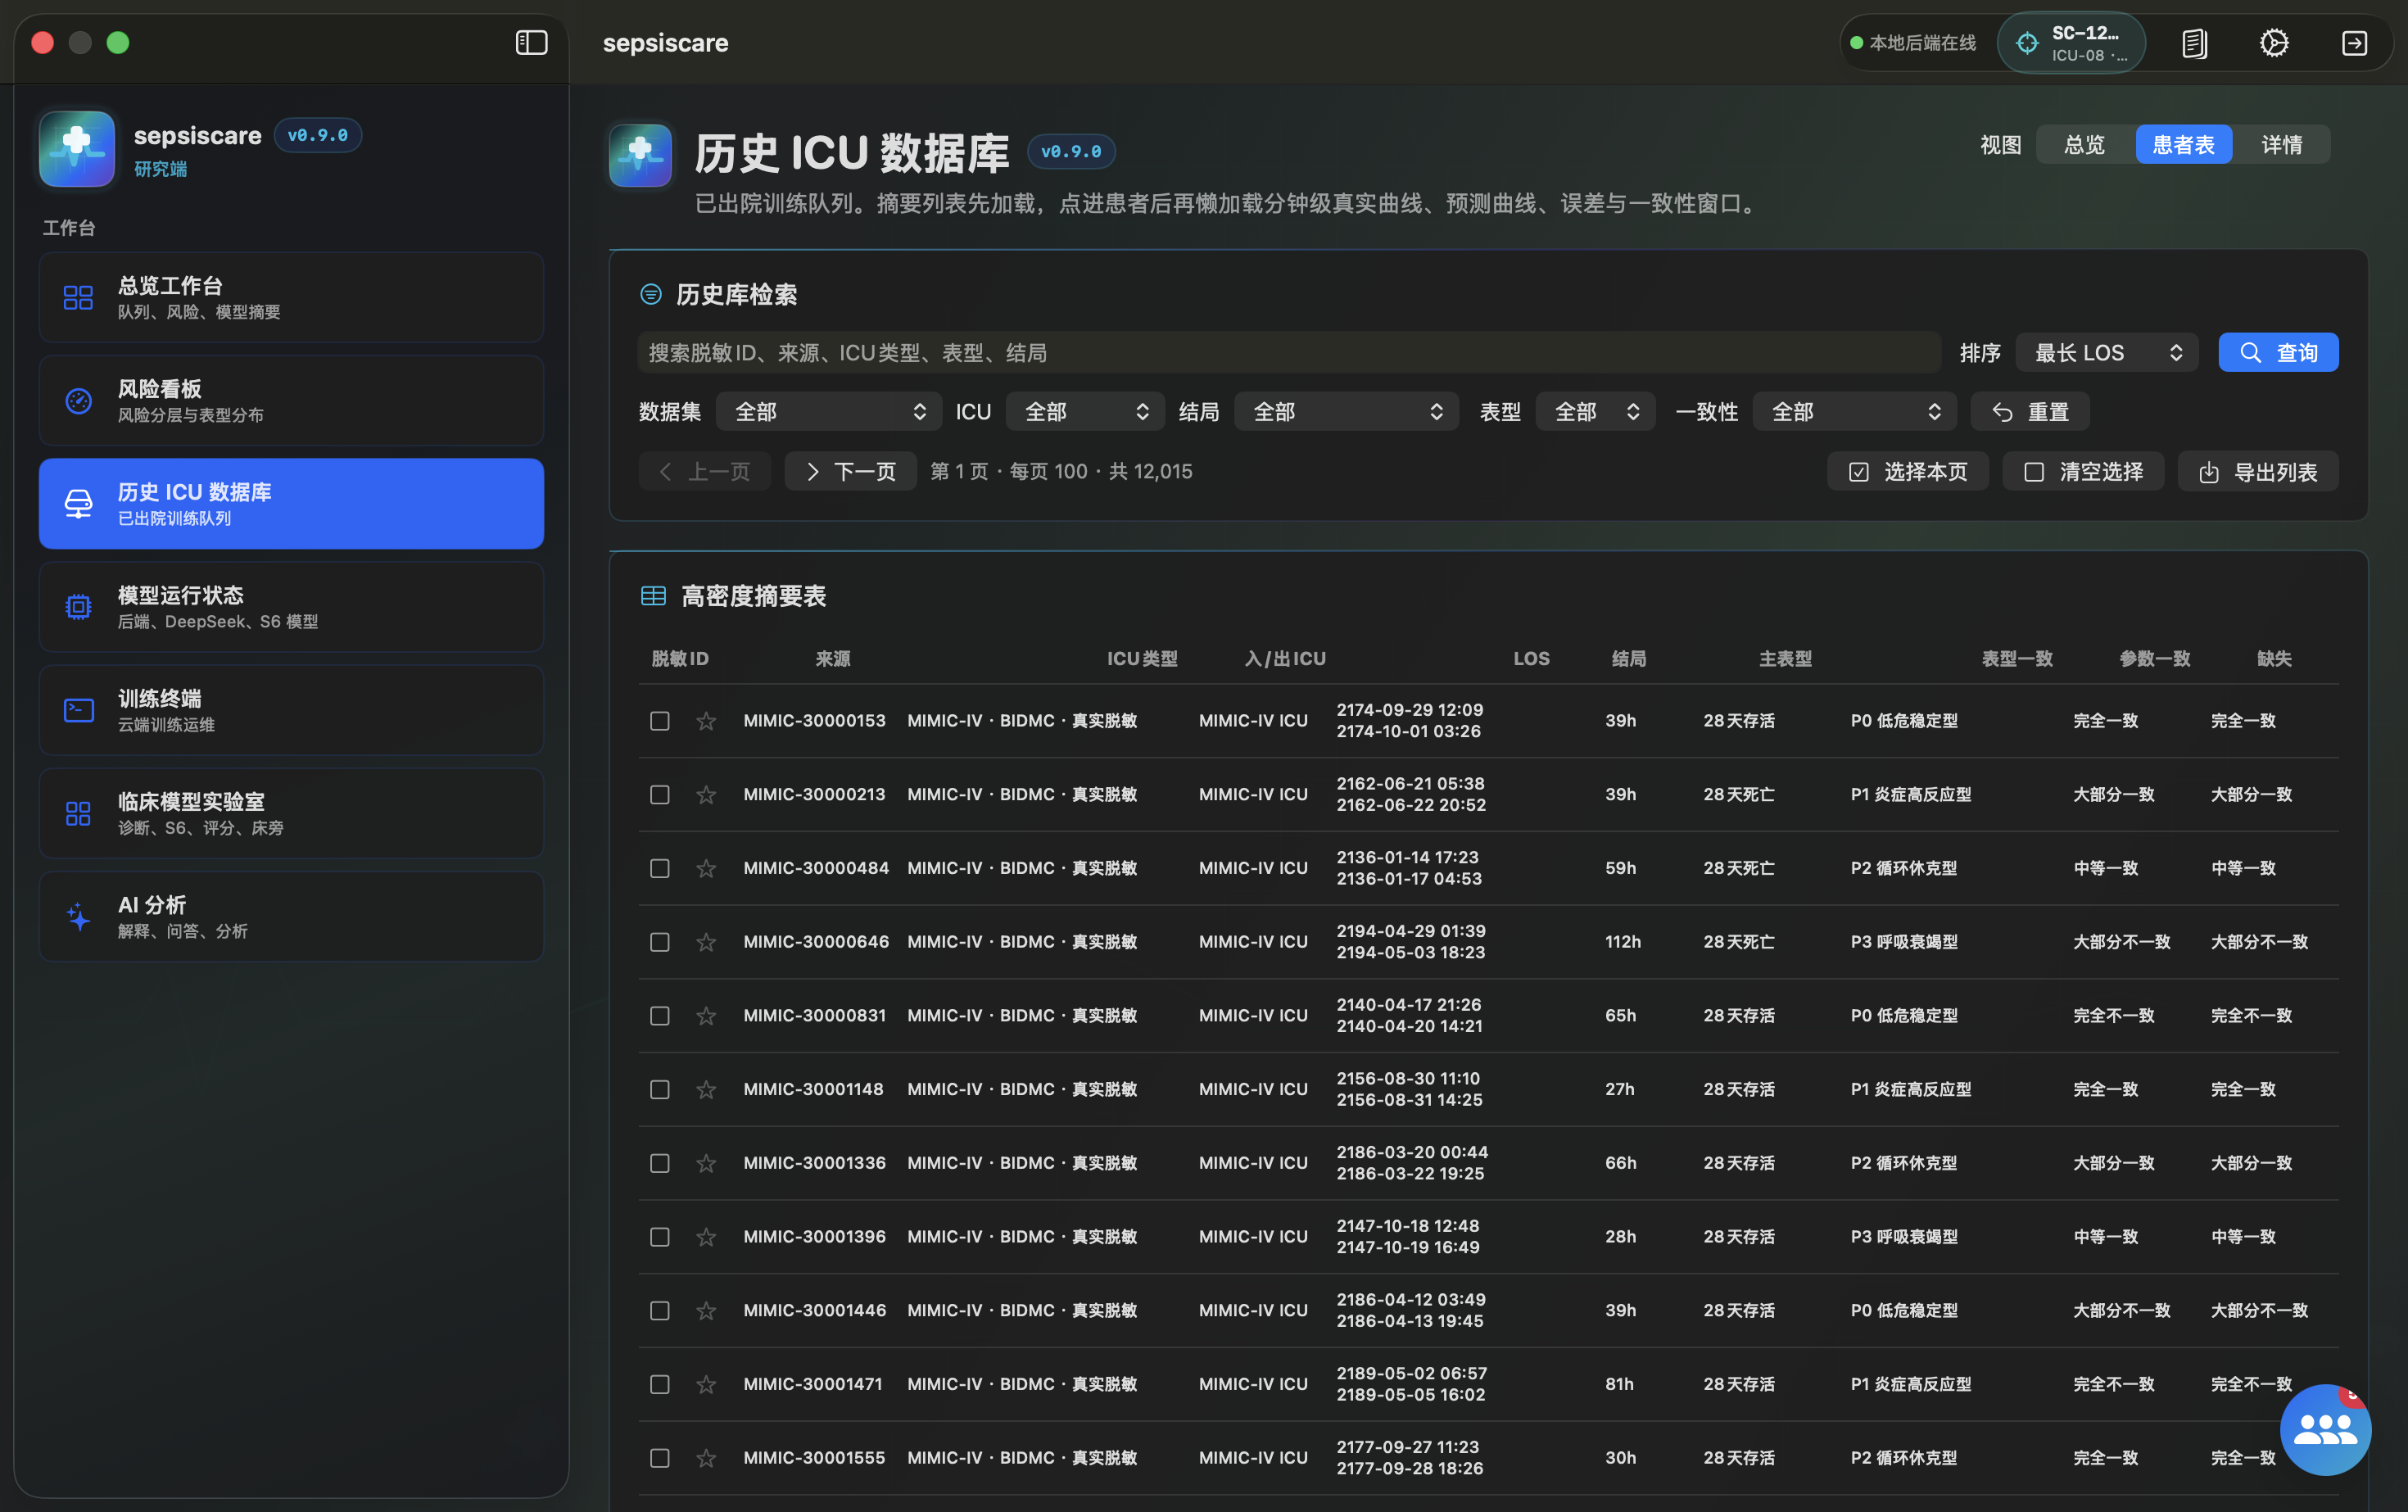
\includegraphics[width=\linewidth]{sepsiscareUI2.png}
\end{minipage}
\caption*{\textbf{软件界面截图。} 左：医生端风险看板与实时趋势；右：研究端历史 ICU 数据库与病例检索。该截图用于说明软件整体功能，不占用正式图号。}
\end{figure}

\clearpage
\subsection{整体架构}
SepsisCare 工程系统采用“多端客户端 + 标准 HTTP API + 可替换本地/云端模型服务”的结构。macOS 和 Windows 安装包内置本地 Python 后端与演示数据；Android 是 WebView 客户端，需要连接本机或云端 API；模型训练终端在演示模式下模拟训练，在生产模式下将命令转发到云端模型服务。图~\ref{fig:software-architecture} 使用新生成的软件架构流程图展示这一分层关系。

\begin{figure}[H]
\centering
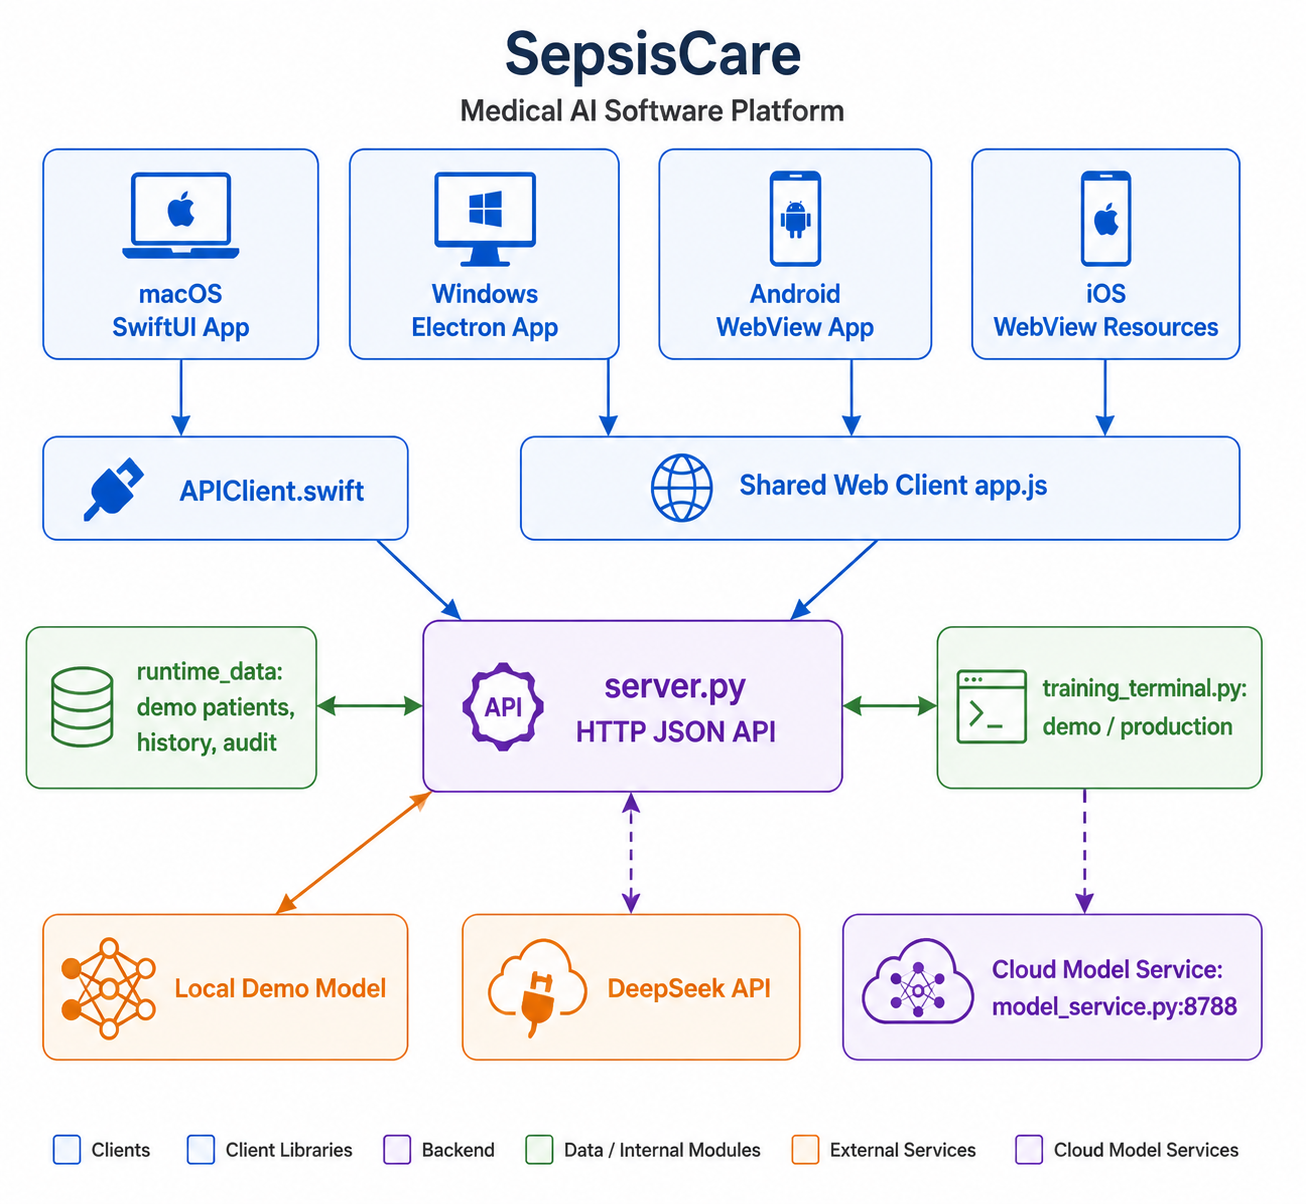
\includegraphics[width=0.92\textwidth]{fig3.png}
\caption{SepsisCare 多端软件架构流程图。macOS、Windows、Android 与 iOS/Web 资源通过统一客户端 API 接入 \texttt{server.py}，后端再连接运行时数据、训练终端、本地演示模型、DeepSeek 与云端模型服务。}
\label{fig:software-architecture}
\end{figure}

\clearpage
\subsection{接口如何运转}
客户端不直接读模型文件，也不直接访问 DeepSeek。所有请求进入 \texttt{server.py}，由后端根据路径分发到患者、历史库、诊断、AI、训练终端等模块。图~\ref{fig:api-flow} 展示了从用户操作到 JSON 响应的完整请求链路。

\begin{figure}[H]
\centering
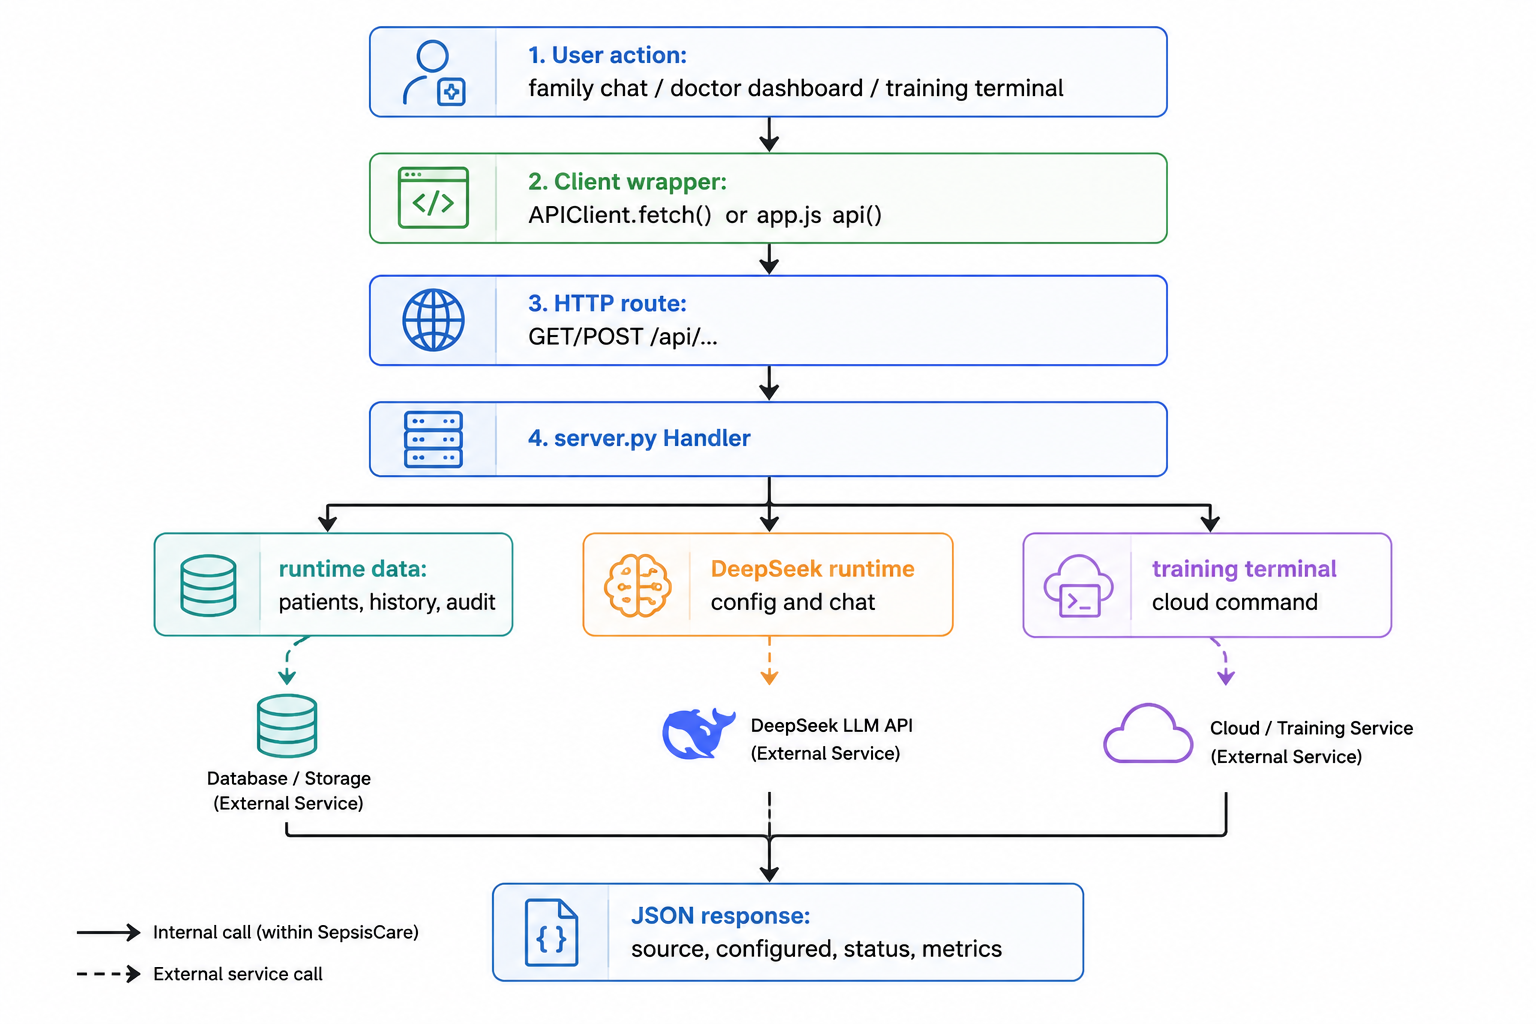
\includegraphics[width=0.96\textwidth]{fig4.png}
\caption{SepsisCare API 请求流转图。用户操作经客户端封装、HTTP 路由和 \texttt{server.py} Handler 后分发至运行时数据、DeepSeek 智能体或训练终端，并统一返回 JSON 响应。}
\label{fig:api-flow}
\end{figure}

\subsection{关键 API 面}
\begin{table}[H]
\centering
\caption{核心 API 路由}
\label{tab:apis}
\reporttablesize
\setlength{\tabcolsep}{5pt}
\renewcommand{\arraystretch}{1.12}
\begin{tabularx}{\textwidth}{@{}l l Y@{}}
\toprule
接口 & 方法 & 作用\\
\midrule
\texttt{/health} & GET & 后端健康检查\\
\texttt{/api/patients} & GET & 当前 ICU 患者列表\\
\texttt{/api/history/patients} & GET & 历史 ICU 病例检索\\
\texttt{/api/model/predict} & POST & 本地模型预测演示\\
\texttt{/api/family/chat} & POST & 家属端智能体沟通\\
\texttt{/api/config/deepseek} & GET/POST & DeepSeek 运行时配置\\
\texttt{/api/training-terminal/status} & GET & 训练终端状态\\
\texttt{/api/training-terminal/action} & POST & 快捷训练动作\\
\texttt{/api/training-terminal/command} & POST & 自定义训练命令\\
\texttt{/api/admin/status} & GET & 管理端服务状态\\
\bottomrule
\end{tabularx}
\end{table}

\subsection{文件结构与相互作用}
最终工程将研究代码、后端、客户端、云端部署包分层，并通过同步脚本和统一 API 保持各端行为一致。文件之间的核心关系如下：
\begin{enumerate}[leftmargin=*,itemsep=1pt]
  \item \texttt{apps/sepsiscare-studio/backend/server.py} 是统一 API 入口，负责患者、历史、模型预测、家属端 AI、训练终端和管理状态接口。
  \item \texttt{apps/sepsiscare-studio/backend/training\_terminal.py} 与业务后端解耦，封装训练动作、远端地址配置、日志回显和演示/生产模式切换。
  \item \texttt{apps/SepsisCare-macOS/Sources/App} 负责 macOS 原生界面、\texttt{APIClient.swift} 请求封装和 \texttt{BackendController.swift} 自动启动后端。
  \item \texttt{apps/sepsiscare-web-client} 是 Windows、Android 与 iOS/Web 资源的共享前端源，构建后同步到 Electron、WebView 与静态资源目录。
  \item \texttt{deploy/sepsiscare\_model\_service/model\_service.py} 是云端模型部署入口，正式生产中由训练终端调用；本地演示模式下使用随安装包分发的轻量后端与示例数据。
  \item \texttt{s6/}、\texttt{s7/} 与 \texttt{scripts/s7\_train\_all\_sources.py} 保存研究训练链路；最终只把必要模型权重、读出器、配置和服务脚本打入模型本体部署包。
\end{enumerate}

\subsection{连接方法}
系统连接方法可以概括为四层：
\begin{enumerate}[leftmargin=*,itemsep=1pt]
  \item \textbf{进程连接：}macOS 后端控制器启动内置 \texttt{server.py}，Windows 主进程启动或连接本地 API，Android/WebView 连接可达 API。
  \item \textbf{协议连接：}统一 HTTP JSON，客户端只关心 endpoint 和 response schema。
  \item \textbf{模型连接：}本地演示走 packaged backend；生产模型走 \texttt{deploy/model\_service.py} 的云端 API。
  \item \textbf{智能体连接：}DeepSeek key 通过 \texttt{/api/config/deepseek} 保存到用户运行时目录，家属端和 AI 端按 \texttt{configured} 状态选择真实调用或本地 fallback。
\end{enumerate}

\FloatBarrier
\section{近期网络安全、防数据污染、系统搭建与部署增量}
\subsection{增量范围与证据边界}
本节回顾上一版报告之后到 2026 年 6 月 3 日之间的工程成果，重点覆盖网络安全、防数据污染、系统搭建和部署四个维度。这里的“成果”只按当前仓库中能被文件、脚本、测试或新鲜命令证明的内容来写：已经实现并验证的内容写成完成项；仍依赖外部机器状态的内容写成阻塞项；课程演示级控制不会被写成 HIPAA、IRB、FDA 或医疗器械合规认证。

\begin{table}[H]
\centering
\caption{近期增量工作的范围、证据和当前边界}
\label{tab:recent-scope}
\reporttablesize
\setlength{\tabcolsep}{4pt}
\renewcommand{\arraystretch}{1.15}
\begin{tabularx}{\textwidth}{@{}l Y Y Y@{}}
\toprule
方向 & 已完成成果 & 主要证据文件/命令 & 仍需保留的边界\\
\midrule
网络安全 & 远端敏感 API fail-closed 鉴权、弱 token 拒绝、SSRF 防护、no-store/nosniff 响应头、Web token 会话化和 URL token 清理 & \path{server.py}、\path{model_service.py}、\path{script/test_web_auth_token.sh}、\path{script/test_demo_auth_boundary.sh} & 不是正式零信任生产网关；远端仍应运行在 Tailscale/VPN/TLS 和密钥轮换体系内\\
防数据污染 & runtime 数据审计、发布面密钥/PHI 审计、训练元数据完整性审计、artifact manifest/HMAC 校验、临床 payload 范围验证 & \path{script/audit_runtime_data.py}、\path{script/audit_sensitive_data.py}、\path{script/audit_training_data_integrity.py}、\path{verify_artifact_bundle.py} & 审计覆盖 release package 和演示 runtime；不替代原始数据治理、恶意样本检测或专家脱敏判定\\
系统搭建 & macOS API/model LaunchAgent、端口占用诊断、远程访问 preflight、Windows/macOS/Linux 一键模型服务入口、Swift/Web/后端测试覆盖 & \path{script/sepsiscare_services.sh}、\path{test_sepsiscare_services.sh}、模型服务 one-click 脚本 & 本机服务和脚本路径已可复现；第二台物理机器仍需单独完成跨机器连通性验证\\
部署编排 & 笔记本到 remote server 的 \path{all/preflight/sync/deploy/smoke/pull-artifacts} 流程、预发布安全门禁、break-glass 跳过审计、artifact 拉回校验 & 本地部署编排脚本、\path{script/pre_release_security_check.sh}、部署编排测试 & remote server 当前 SSH 仍关闭连接，远端实际部署不能写成已完成\\
\bottomrule
\end{tabularx}
\end{table}

\subsection{网络安全加固}
网络安全工作的核心变化，是把原来偏演示友好的“本地服务可直接访问”改为分层边界：本机 loopback 仍然便于开发和课堂演示，远端敏感 API 则必须配置 Bearer token；token 不存在、过弱或缺失时全部 fail closed；会触发训练、artifact、审计、历史导出、DeepSeek 配置和远程模型管理的接口都被纳入敏感面。这个设计避免了把前端登录密码 \texttt{123123} 误当成远端 API 鉴权，也避免了把训练终端、artifact 下载和审计日志暴露给同网段未授权客户端。

\begin{table}[H]
\centering
\caption{网络安全控制矩阵}
\label{tab:network-security-controls}
\scriptsize
\setlength{\tabcolsep}{3pt}
\renewcommand{\arraystretch}{1.14}
\begin{tabularx}{\textwidth}{@{}l Y Y Y@{}}
\toprule
控制点 & 实现方式 & 被保护的风险 & 验证/证据\\
\midrule
远端敏感 API 鉴权 & \texttt{SEPSISCARE\_SERVICE\_TOKEN} 或 \texttt{SEPSISCARE\_TRAINING\_TOKEN}；远端未配置、弱 token、缺失/错误 Bearer 分别返回 403/403/401 & 防止训练命令、artifact、审计和敏感历史接口被局域网或 VPN 内未授权客户端调用 & \path{apps/sepsiscare-studio/backend/server.py}、\path{02_model_deploy_package/deploy/model_service.py}、\path{test_model_service.py}\\
本地/远端边界 & loopback 继续可用；远端访问需要 token；本地服务默认文档强调 \texttt{127.0.0.1}，只有可信网络才显式 \texttt{0.0.0.0} & 避免课堂演示便利性直接变成远端暴露面 & \path{TRANSFER_README.md}、\path{README_DEPLOY.md}\\
训练服务 URL 约束 & \texttt{cloud\_base\_url} 保存和转发前规范化，只接受 HTTP(S) 模型服务地址，拒绝 metadata、link-local、multicast、reserved、credential-bearing URL & 防止训练终端成为 SSRF 或凭据泄漏通道 & \path{server.py}、\path{model_service.py}、后端单测\\
响应头与文档面 & 敏感响应设置 \texttt{Cache-Control: no-store} 与 \texttt{X-Content-Type-Options: nosniff}；远端 FastAPI docs/Redoc 禁用 & 减少浏览器缓存、MIME sniffing 和自动文档暴露风险 & \path{model_service.py}、\path{server.py}\\
Web token 存储 & Web/Windows/iOS/Android 共享前端不再把 API token 持久化到 \texttt{localStorage}，只保留本次会话；历史 token 启动时移除 & 减少长期浏览器存储、截屏、拷贝和共享电脑遗留风险 & \path{script/test_web_auth_token.sh}\\
HTML 输出转义 & 对患者、历史、chat、audit、绑定、状态、终端输出等服务端返回文本进行 escaping 后进入 \texttt{innerHTML} & 降低被污染后端响应导致的 XSS/content injection 风险 & \path{script/test_web_content_escape.sh}\\
演示登录边界 & \texttt{123123} 被文案和测试固定为客户端演示门，不再被描述为生产鉴权 & 防止将课堂演示密码误用为远端 API 安全机制 & \path{script/test_demo_auth_boundary.sh}\\
\bottomrule
\end{tabularx}
\end{table}

\subsection{防数据污染、脱敏与发布完整性}
防数据污染这部分从四个层面建立门禁。第一层是运行时患者数据：发布包和本地后端的 \path{runtime_data} 需要通过 provenance、masked id、直接标识字段、敏感文本、重复标识、孤立 detail series 和临床数值范围检查。第二层是发布文件面：模型包、后端、Web、Windows、iOS 和 Android 静态资源会扫描高置信密钥和 PHI-like 文本，结果只输出文件、行号和短哈希，不回显敏感原文。第三层是训练元数据：检查四个来源、训练总人数、split policy、目标 run、指标范围，避免把全量重叠监控切分误写成 held-out 外部验证。第四层是 artifact：下载包在服务端按已知模型/报告根目录重新构建，排除 runtime logs、配置文件、symlink，并写入 \texttt{MANIFEST.sha256} 和可选 \texttt{MANIFEST.sha256.hmac}。

\begin{table}[H]
\centering
\caption{防污染与脱敏控制矩阵}
\label{tab:data-pollution-controls}
\scriptsize
\setlength{\tabcolsep}{3pt}
\renewcommand{\arraystretch}{1.14}
\begin{tabularx}{\textwidth}{@{}l Y Y Y@{}}
\toprule
层级 & 控制内容 & 阻断/降低的风险 & 当前验证结果\\
\midrule
运行时历史数据 & 必填 5 个 provenance 字段，删除 subject/hadm/MRN/DOB/name/address 等直接标识字段，detail rows 只保留临床时间序列 & 原始患者标识混入演示数据库、孤立 detail 数据、异常数值直接进入发布包 & 部署包和本地后端两个副本均为 12015 patients、720 detail rows、0 fatal violations、261 display-summary warnings\\
敏感发布面 & 六个 release surface 扫描高置信 API key/token/Bearer header 和 PHI-like 文本；测试、模型二进制、图片、报告等按规则排除 & 硬编码密钥、PHI-like 文本或复制的 token 被提交到可发布目录 & 6 roots、0 findings\\
训练元数据 & 检查来源 provenance、full-overlap 监控切分、声明训练人数、目标 run 和指标范围 & 把 all-source monitoring split 误宣传成外部 held-out 验证；训练人数或指标被污染 & 4 sources、347634 declared train patients、1 target run row、0 violations\\
临床 payload & 预测/诊断请求拒绝非数值或越界临床值，batch diagnosis 上限 20 个 patient object & 恶意或格式错误 payload 影响模型输出、日志和前端展示 & \path{test_model_service.py} 与 \path{test_server.py} 覆盖\\
外部 LLM prompt & 递归清洗 sensitive keys、MRN/email/phone/DOB/SSN、patient/bed/history ids，限制 prompt 深度、列表长度和文本长度 & 家属端或 AI 解释把内部患者标识/敏感值送到外部 LLM & \path{model_service.py}、\path{server.py} 实现并在安全综述中记录\\
Artifact 完整性 & ZIP 中包含 \texttt{MANIFEST.sha256}，可选 \texttt{MANIFEST.sha256.hmac}；验证器检查路径安全、逐文件 SHA256 和 HMAC & 陈旧 artifact、symlink 间接携带 secret、下载后内容被替换或损坏 & \path{test_verify_artifact_bundle.py}、\path{verify_artifact_bundle.py}\\
\bottomrule
\end{tabularx}
\end{table}

\begin{table}[H]
\centering
\caption{2026-06-03 报告更新前重新运行的关键审计摘要}
\label{tab:fresh-audit-summary}
\reporttablesize
\setlength{\tabcolsep}{5pt}
\renewcommand{\arraystretch}{1.12}
\begin{tabularx}{\textwidth}{@{}l r r r Y@{}}
\toprule
检查项 & 对象数 & 错误/发现 & 警告 & 结论\\
\midrule
部署包 runtime 数据审计 & 12015 patients / 720 detail rows & 0 fatal violations & 261 & 通过；警告来自展示摘要字段，不阻塞 release，但应在受监管部署前清理\\
本地后端 runtime 数据审计 & 12015 patients / 720 detail rows & 0 fatal violations & 261 & 通过；与部署包副本一致\\
六个发布面敏感数据审计 & 6 roots & 0 findings & 0 & 通过；未发现高置信硬编码密钥或 PHI-like 文本\\
训练元数据完整性审计 & 4 sources / 347634 train patients & 0 violations & 0 & 通过；目标 S7 run 存在，指标范围和 split policy 未发现污染\\
Remote server SSH preflight & 1 host & SSH closed connection & -- & 未通过；说明远端实际部署仍受 remote server 主机连通性阻塞\\
\bottomrule
\end{tabularx}
\end{table}

\subsection{系统搭建与部署编排}
系统搭建从“单机可运行”扩展为“本机 API + 模型服务 + remote server 编排 + 拉回 artifact”的闭环。当前项目中有三组入口：\path{script/sepsiscare_services.sh} 负责本机或目标 macOS 上的 API/model 服务启动、状态、smoke、LaunchAgent 安装和卸载；模型包中的 Linux/macOS one-click 脚本负责 remote server 上的 doctor/start/restart/status/smoke/logs；本地部署编排脚本负责从我的笔记本侧完成预发布检查、SSH preflight、rsync 同步、远端重启、笔记本到 remote server smoke 和 artifact 拉回。需要强调的是，本轮实验与验证均在我的笔记本上完成；真正 remote server 的独立端到端部署仍等待远端主机恢复 SSH 与跨机器 smoke 证据。

\begin{table}[H]
\centering
\caption{系统搭建与部署能力清单}
\label{tab:deployment-capabilities}
\scriptsize
\setlength{\tabcolsep}{3pt}
\renewcommand{\arraystretch}{1.14}
\begin{tabularx}{\textwidth}{@{}l Y Y@{}}
\toprule
能力 & 当前实现 & 价值\\
\midrule
本机服务管理 & \path{script/sepsiscare_services.sh} 支持 start/stop/status/smoke/install-agent/uninstall-agent，状态输出实际监听地址、loopback/remote-capable 解释和远程检查命令 & 新电脑恢复时能快速判断服务是否在线、端口是否被占用、是否可从另一台电脑访问\\
远端模型服务启动 & Linux/macOS 使用 one-click model-service 脚本，Windows 使用 \path{start_model_service_windows.ps1}，doctor/start/restart 前均运行 runtime data audit & 避免把污染的 runtime 数据服务化；保留跨平台模型服务入口\\
笔记本到 remote server 一键编排 & 本地 all 流程串联预发布安全检查、SSH、审计、rsync、远端 restart/smoke、笔记本侧 forwarding smoke、artifact 下载 & 部署从手工命令集合变成可测试流程，降低遗漏检查的风险\\
预发布安全门禁 & \path{pre_release_security_check.sh} 汇总 audit 单测、真实数据审计、敏感发布面审计、训练元数据审计、model-service/backend/web/deploy/services/Swift 构建检查 & 把网络安全、防污染、部署脚本和多端客户端安全测试放在同一个 release gate 中\\
Artifact 拉回与校验 & \path{pull-artifacts} 下载 \texttt{sepsiscare\_model\_artifacts\_latest.zip}；当配置 \texttt{SEPSISCARE\_ARTIFACT\_SIGNING\_KEY} 时自动运行 verifier & 让部署后产物能被 Mac 侧保存、复核和交付，不只依赖远端口头成功\\
当前 remote server 状态 & 2026-06-03 重新执行 SSH preflight，返回 \texttt{Connection closed by 198.18.1.225 port 22} & 远端脚本路径已就绪，但 remote server 仍不可写成实际部署完成\\
\bottomrule
\end{tabularx}
\end{table}

\subsection{近期验证闭环}
安全综述 \path{SECURITY_PRIVACY_ETHICS_REVIEW.md} 记录了一次完整加固后的验证组合，包括 model service 单测、artifact verifier 单测、runtime/sensitive/training audit 单测、本地后端单测、Web token/demo-auth/content escaping/syntax 检查、部署文档 secret hygiene、笔记本到 remote server 编排测试、服务编排测试、remote server one-click smoke 和 Swift build。报告更新前又重新运行了四个关键审计与 remote server preflight，结果见表~\ref{tab:fresh-audit-summary}。因此，本节的完成边界是：网络安全和防污染控制已经进入代码、测试和部署门禁；本机与脚本级部署链路可复现；remote server 远端实际执行仍等待主机在线、SSH 可用和跨机器 smoke。

\FloatBarrier
\section{软件交付结果}
最终交付物分为三类：第一类是软件客户端交付，包括已生成的 macOS DMG，以及 Windows、Android、iOS 与 Web 客户端源码和构建脚本；第二类是独立模型本体与 remote server 部署包，包含 S7 模型、读出器、训练摘要、remote server 模型服务和一键启动脚本；第三类是全套使用文档，包括安装向导、训练终端教程、部署说明、论文式报告、最终答辩 PPT 与哈希校验表。软件、模型与文档分离，可以避免把大型原始数据或敏感 API key 打入安装包，也便于在课程演示与正式投产之间切换部署策略。2026 年 6 月 3 日增补后，交付物还包括安全/隐私/伦理综述、预发布安全门禁、runtime 数据审计器、发布面敏感数据审计器、训练元数据完整性审计器、artifact bundle verifier，以及笔记本到 remote server 的可测试部署编排流程。

\section{结论}
SepsisCare 完成了从 ICU 时间序列研究到多端软件系统的完整课程项目闭环。研究侧，S0--S7 逐步解决了数据标准化、自监督表示、动态表型、跨中心验证、实时部署校准、多源轨迹编码和最终表型监督模型问题。工程侧，系统形成了可安装客户端、内置后端、运行时 DeepSeek 配置、训练终端、remote server 模型部署包、预发布安全门禁和最小最终交付目录。近期安全加固把远端敏感 API、Web token、SSRF、XSS、运行时数据、训练元数据、artifact 完整性和部署流程纳入同一条证据链，使系统从“能演示”进一步接近“能复现、能审计、能解释边界”的课程级交付。最终模型指标适合课程演示、答辩展示和工程验收，但不应被表述为临床级外部验证；当前 remote server 部署也只能写成编排路径就绪，不能写成远端已经完成。

\section{下一步工作}
后续工作包括：
\begin{enumerate}[leftmargin=*,itemsep=1pt]
  \item 建立真正 held-out 外部验证切分，避免 S7 监控切分与训练重叠。
  \item 加入源条件读出器或非泄漏 readout adaptation，针对 eICU 等困难域提升表型一致性。
  \item 将云端训练服务接入任务队列、鉴权、日志持久化和模型版本管理。
  \item 将本地演示历史数据导入/导出流程标准化，使新电脑安装后可恢复用户历史。
  \item 对 DeepSeek 智能体加入提示词版本、离线 fallback 和更多临床边界测试；现有外部 LLM prompt 脱敏与 URL 约束仍需在更大样本上压力测试。
  \item 完成正式代码签名、公证、Windows SmartScreen 信誉积累和 Android release signing。
  \item 在 remote server 重新上线后执行笔记本到远端的一键部署流程，保存远端 smoke、artifact verifier 和跨机器访问证据。
  \item 清理 runtime audit 中 261 个 \texttt{\_detail\_profile} 展示摘要警告；这些不是 release fatal blocker，但受监管部署前应完成数据治理复核。
  \item 在获得明确授权后运行仓库级 Codex Security 深度扫描，并把 threat model、攻击面路径和修复记录并入安全综述。
\end{enumerate}

\section*{交付与复现说明}
本报告对应最终目录：
\begin{lstlisting}
/Users/exusiaihy/SepsisCare_macOS_app_model_transfer_20260528/
  SepsisCare_Final_Delivery_20260603.zip
  outputs/final_delivery/SepsisCare_Final_Delivery_20260603/
    01_documentation/
    02_installers/
    03_remote_server_model_package/
    04_client_source/
    05_quality_security/
    06_scripts/
    SHA256SUMS.txt
\end{lstlisting}
DeepSeek API Key 不写入报告、源码或安装包；新机器安装后需通过软件设置页或管理员端服务监控页填写。

\begingroup
\raggedright
\begin{thebibliography}{99}
\bibitem{ieee-template}
IEEE Author Center, ``IEEE Article Templates,'' accessed 2026-05-19. [Online]. Available: \url{https://template-selector.ieee.org/}
\bibitem{acm-template}
Association for Computing Machinery, ``ACM Primary Article Template,'' accessed 2026-05-19. [Online]. Available: \url{https://www.acm.org/publications/proceedings-template}
\bibitem{sepsis3}
M. Singer et al., ``The Third International Consensus Definitions for Sepsis and Septic Shock (Sepsis-3),'' \emph{JAMA}, 2016.
\bibitem{physionet2012}
M. Saeed et al., ``Multiparameter Intelligent Monitoring in Intensive Care II (MIMIC-II): a public-access intensive care unit database,'' \emph{Critical Care Medicine}, 2011; PhysioNet Challenge 2012 data interface used in this project.
\bibitem{physionet2019}
M. A. Reyna et al., ``Early Prediction of Sepsis from Clinical Data: the PhysioNet/Computing in Cardiology Challenge 2019,'' \emph{Critical Care Medicine}, 2020.
\bibitem{mimiciv}
A. E. W. Johnson et al., ``MIMIC-IV, a freely accessible electronic health record dataset,'' \emph{Scientific Data}, 2023.
\bibitem{eicu}
T. J. Pollard et al., ``The eICU Collaborative Research Database, a freely available multi-center database for critical care research,'' \emph{Scientific Data}, 2018.
\bibitem{transformer}
A. Vaswani et al., ``Attention Is All You Need,'' NeurIPS, 2017.
\bibitem{gru}
K. Cho et al., ``Learning Phrase Representations using RNN Encoder--Decoder for Statistical Machine Translation,'' EMNLP, 2014.
\bibitem{grud}
Z. Che et al., ``Recurrent Neural Networks for Multivariate Time Series with Missing Values,'' \emph{Scientific Reports}, 2018.
\bibitem{supcon}
P. Khosla et al., ``Supervised Contrastive Learning,'' NeurIPS, 2020.
\bibitem{groupdro}
S. Sagawa et al., ``Distributionally Robust Neural Networks for Group Shifts,'' ICLR, 2020.
\bibitem{coral}
B. Sun and K. Saenko, ``Deep CORAL: Correlation Alignment for Deep Domain Adaptation,'' ECCV Workshops, 2016.
\bibitem{dml}
V. Chernozhukov et al., ``Double/debiased machine learning for treatment and structural parameters,'' \emph{The Econometrics Journal}, 2018.
\end{thebibliography}
\endgroup

\end{document}
